\documentclass[a4,center,fleqn]{NAR}

% Enter dates of publication
\copyrightyear{2018}
\pubdate{31 July 2019}
\pubyear{2019}
\jvolume{00}
\jissue{00}

%\articlesubtype{This is the article type (optional)}

\begin{document}

\title{PconsFam: A regularly updated database of structure predictions of all Pfam families available at http://pconsfold.bioinfo.se/}

\author{%
John Lamb\,$^{1,*}$,
Aleksandra Jarmolińska\,$^{2,*}$
Mirco Michel\,$^{1,*}$,
David Menéndez-Hurtado\,$^{1,*}$,
Joanna Sułkowska,$^{2,\dagger}$
Arne Elofsson\,$^{1,\dagger}$%
\footnote{To whom correspondence should be addressed.
Tel: +46 706951045; Email: arne@bioinfo.se}}

\address{%
$^{1}$Science for Life Laboratory and Department of Biochemistry and
biophysics, Stockholm Unviersity, Tomtebodav 23, 171 21 Solna, Sweden
and
$^{2}$ Warsaw, Poland 
$^{*}$ contributed equally
$^{\dagger}$=contributing authors
% Affiliation must include:
% Department name, institution name, full road and district address,
% state, Zip or postal code, country
}

\history{%
Received January 1, 2019;
Revised February 1, 2019;
Accepted March 1, 2019}

\maketitle





\begin{abstract}


\end{abstract}

\section{Introduction}

In recent years it has been shown that by the use of evolutionary
information and direct coupling analysis~\cite{Weigt19116270} it is
possible to obtain sufficiently accurate contact prediction of
proteins from their sequence and multiple sequence alignment alone to
predict accurate structures of many protein
families~\cite{Sulkowska2012}. At first the DCA methods were limited
to very large protein families, but with the use of deep learning
methodologies to improve the contact predictions it is nowadays
possible to accurately predict the contacts for families with only a
few hundred members~\cite{Skwark25375897,Michel28535189,Wang28056090}

Using these predicted contacts it is then possible to model the
structure of a protein using a protein folding program. Here,
initially CNS was used ~\cite{Morcos22106262} but Rosetta has also
been used~\cite{Baker:1999}. Although it is possible that models
created by Rosetta are of slighlty higher quality than models by
CNS~\cite{Michel25161237} the advantagae of CNS is clear as it is much
faster. 


Recently we developed the PconsFold2 pipeline~\cite{Michel28881974}, which uses contact
predictions from PconsC3~\cite{Michel28535189} the CNS based CONFOLD folding
algorithm~\cite{Adhikari25974172} and most importantly multiple model quality estimations
\cite{Uziela28052925,Lundstrom:2001} to predict the structure of
proteins. Here we present the related web resource PconsFam
(https://pconsfam.bioinfo.se) a database with predicted structural
information for most Pfam families using the PconsFold2
pipeline.


The PconsFold2 pipeline can predict accurate models (TM-score $>0.5$
for 51\% of the large families ($>1000$ effective sequences). For
smaller families the fraction of correct models decreases, bu they
still exist. Therefore, a major challenge for large scale predictions
is to distinguish between correct and incorrect models. Here, we have
applied a set of model quality estimation methods~\cite{Kryshtafovych28833563}.


\bf{(ADD MORE NUMBERS)}


When the PconsFold2 pipeline was applied to 6379 PFAM families of
unknown structure 558 modes with a predicted specificity over 90\% was
created. Out of these, 415 had never been reported before.

{\bf With
PconsFam we extend this pipeline to the full PFAM database to predict
multiple contact maps and subsequently multiple structures of all
representative sequences for all Pfam families. }

For each family in
PFAM, multiple contact maps are generated and from these a set of
models are predicted and ranked with quality assessment
estimators. The model quality estimation gives an indication on the
reliability of the model. The top ranked models for each predicted
family can be visualised and are available for download. The full set
of contact predictions for is available for visualisation together
with the predicted model in an intuitive and powerful user-interface
that allows interaction between the contact maps and the predicted
structure. 

\section{Material and methods}
\subsection{PconsFold2}
We have used 

PconsC4
CONFOLD

\subsection{Model Quality assessment}
Pcons
ProQ4
PPV
Known PDB structures

\subsection{Updates}

With our pipeline the website will be updated with every PFAM release
and the currently running update on PFAM 31.0 will introduce
additional quality estimators such as PPV, Pcons score and ProQ4
scores. 

\section{Results}

\subsection{Comparison with other resources}

A similar resource is Baker Lab’s GREMLIN database~\cite{Kamisetty2013} which builds contact prediction based on
PFAM 27.0~\cite{Sonnhammer:1997} . However, it has not been updated since
2013. In contrast we plan to update PconsFam within a few month after
each Pfam release. This is possible as the pipeline uses a much less
computationally costly methodology. PconsC4 is at least one order of
magnitude faster than comparative methods and by using CONFOLD the
folding is much faster than Rosetta.


GREMLIN shows predicted contact maps with an option to overlay with
the pdb structure if one exists. We extend on this by using a tool
that can visualize the predicted contacts on the models. In our
database, both contact maps and predicted structure can be
investigated in detail and downloaded.  We have also used a deep
learning methodology (currently PconsC3 but will be updated to PconsC4
before publication) for contact predictions. In general this provide
the better coverage of small protein families.




\begin{figure}[t]
\begin{center}
\end{center}
\caption{PconsC3/4 vs DCA
ProQ evaluations 
The PconsFold pipeline.}
    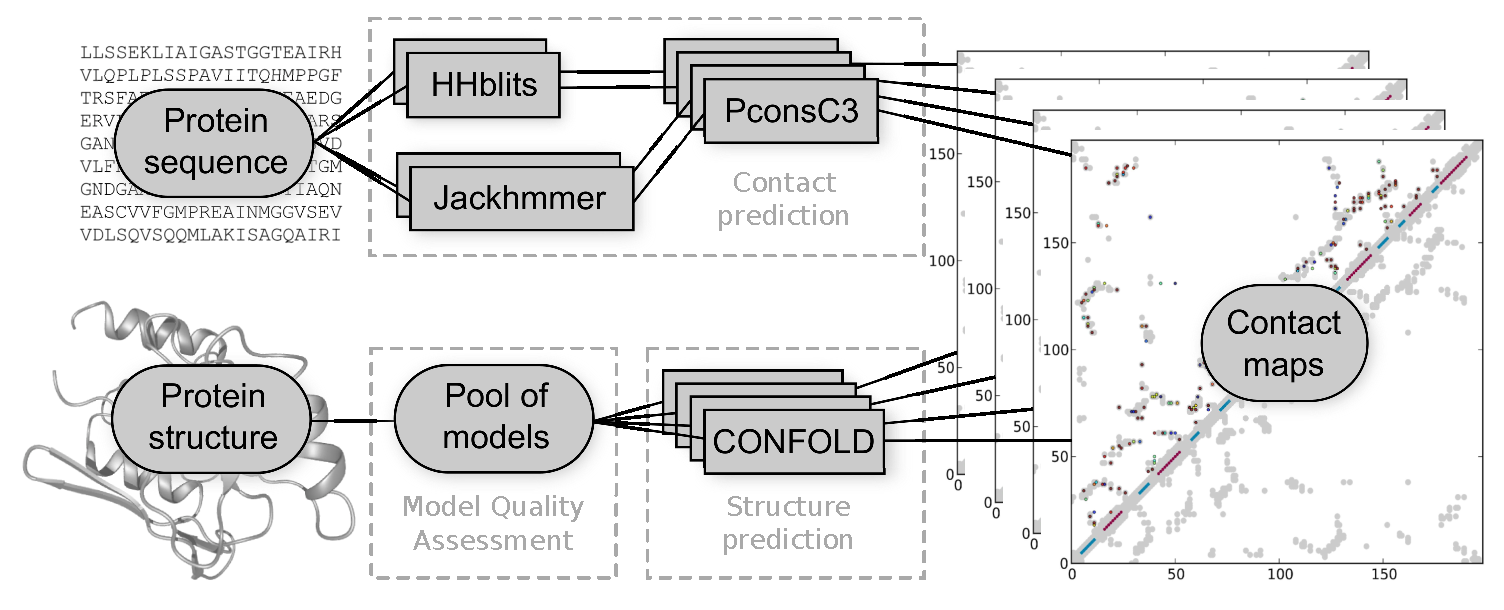
\includegraphics[width=0.5\textwidth]{figures/flowchart.eps}
\label{fig:Pipeline}
\end{figure}


\begin{figure}[t]
\begin{center}
\end{center}
\caption{Comparison of contact prediction methods and available resources
Comparison of databases of structure predictions
Gremlin
EV-fold ?
Zhang ?.}
    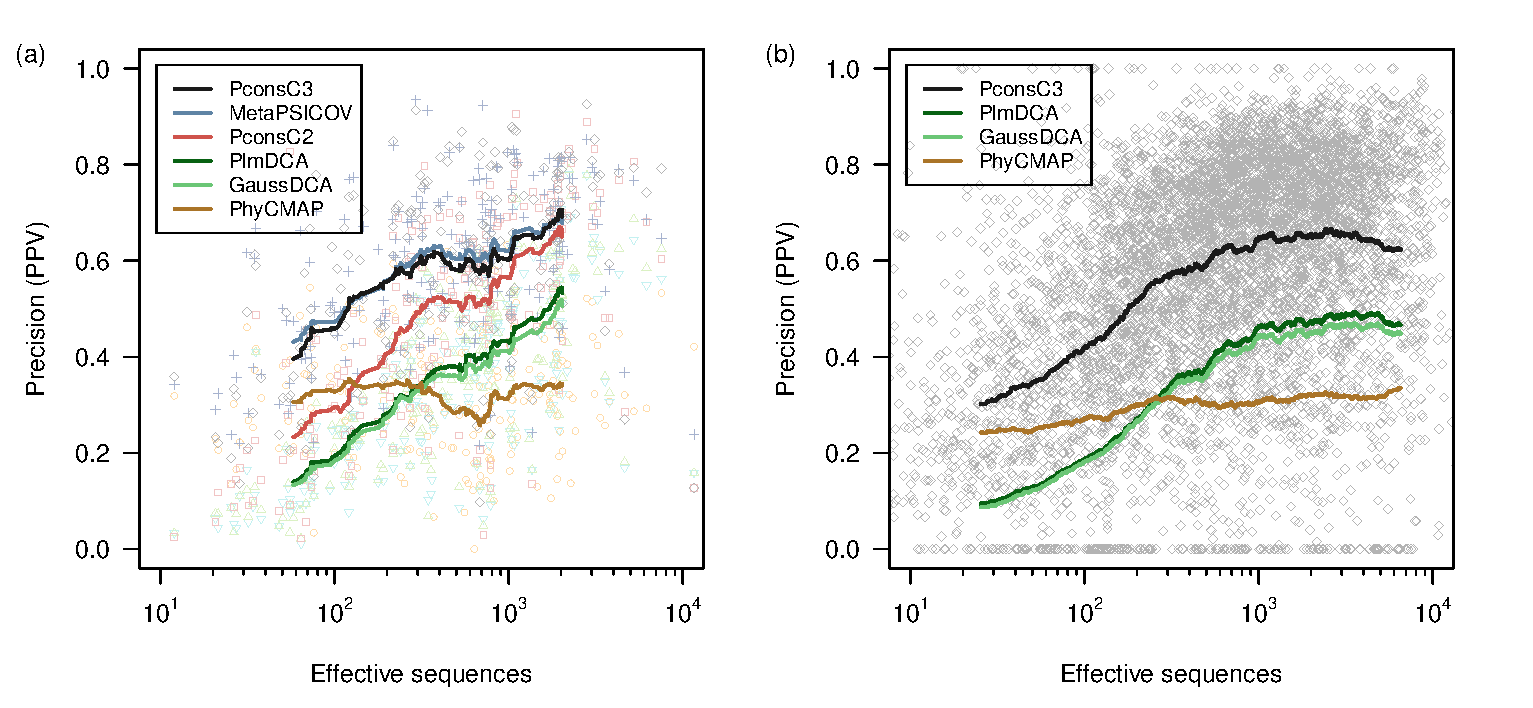
\includegraphics[width=0.5\textwidth]{figures/fig1_PNAS.eps}
\label{fig:comparison}

\end{figure}
\begin{figure}[t]
\begin{center}
\end{center}
\caption{Comparison of contact prediction methods and available resources
Comparison of databases of structure predictions
Gremlin
EV-fold ?
Zhang ?.}
    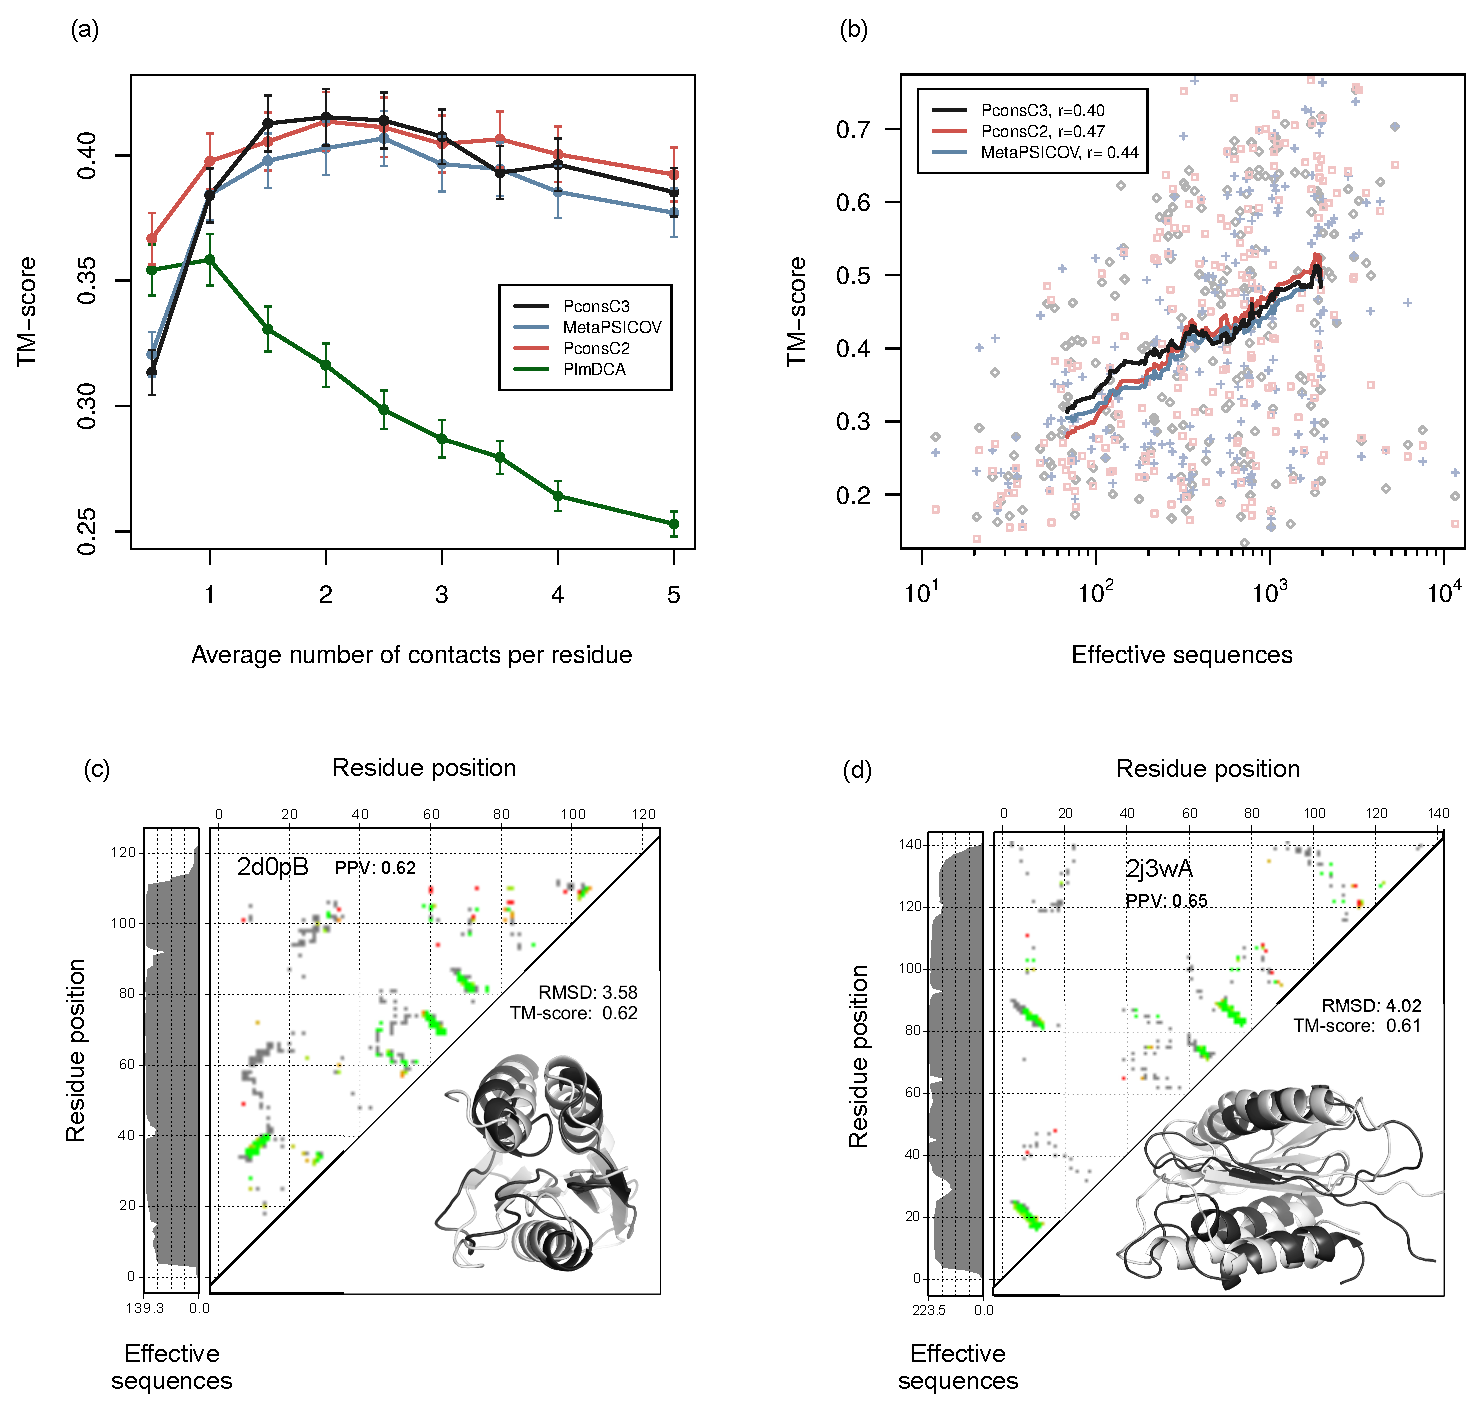
\includegraphics[width=0.5\textwidth]{figures/fig4_PNAS.eps}
\label{fig:comparison}
\end{figure}


\begin{figure}[t]
\begin{center}
\end{center}
\caption{Overview of number of structures at different qualities - from PconsFold
verview of the database.}
    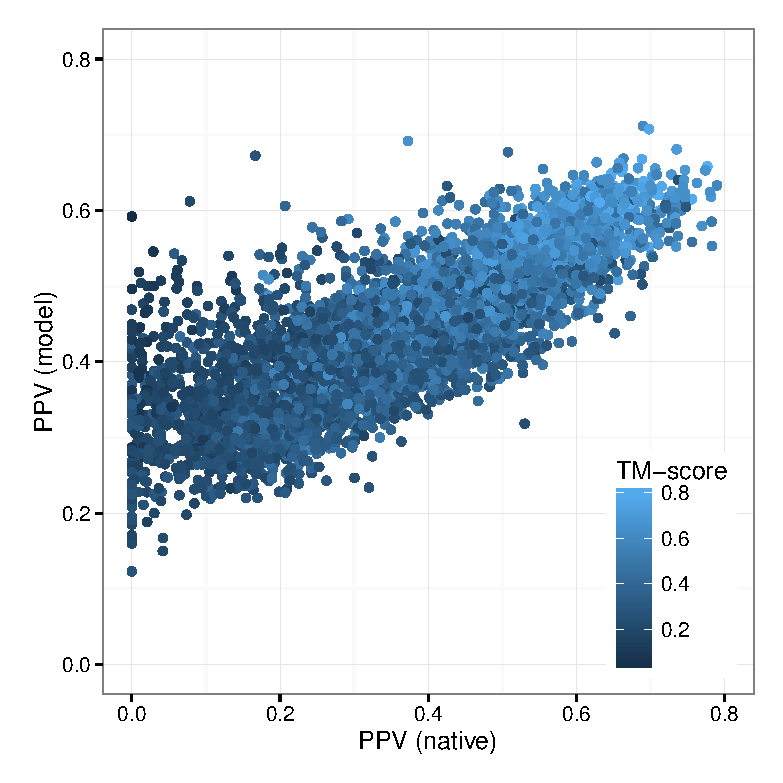
\includegraphics[width=0.5\textwidth]{figures/fig_pfam_ppv_native_vs_model.eps}
\label{fig:overview}
\end{figure}


\begin{figure}[t]
\begin{center}
\end{center}
\caption{Links Knots - topology.}
\label{fig:Interface}
\end{figure}


\begin{figure}[t]
\begin{center}
\end{center}
\caption{.}
\label{fig:exampel PF0009.24}
\end{figure}


\begin{table}[t!]
\centering
\caption{Average PPV of top $N/2$ predicted contacts on the benchmark dataset for different secondary structural classes. \label{tab:ss}}
%{\begin{tabular}{lp{1cm}p{1cm}p{1cm}p{1cm}p{1cm}p{1cm}}\toprule
{\begin{tabular}{lcccc}
  \hline
 & all & mainly-$\alpha$ & mainly-$\beta$ & $\alpha-\beta$ \\ 
  \hline
  PconsC3 & 0.57 & 0.49 & 0.59 & 0.62 \\ 
    MetaPSICOV & 0.59 & 0.54 & 0.58 & 0.62 \\ 
    PconsC2 & 0.48 & 0.44 & 0.45 & 0.51 \\ 
    PlmDCA & 0.36 & 0.34 & 0.32 & 0.38 \\ 
    GaussDCA & 0.34 & 0.33 & 0.31 & 0.36 \\ 
    PSICOV & 0.34 & 0.30 & 0.33 & 0.35 \\ 
    PhyCMAP & 0.32 & 0.23 & 0.34 & 0.36 \\ 
   \hline
  counts & 210 & 55 & 35 & 110 \\
   \hline
\end{tabular}}{}
\end{table}


\begin{table*}[tb!]
\centering
\caption{Properties of Pfam families that can be modeled accurately at FPR
0.1. Statistical significant differences
from a students t-test at P-values 0.01 and $10^{-5}$ are marked with $^*$ and
$^{**}$ respectively for all columns except the last.}

\label{tab:nopdb2}
\begin{tabular}{lllllllll}
  \hline
  & PconsC3 score & Helix & Sheet & Coil & Meff & Length & Transmembrane & TM-score\\ 
  \hline
  %ProQ3D & 0.64 & 0.5$^{**}$ & 0.47$^{**}$ & 0.1$^{**}$ & 0.42$^{**}$ & 375.72$^{**}$ & 102.6$^{**}$ & 0.07$^{**}$ \\ 
  %PcombC & 0.55 & 0.62$^{**}$ & 0.35 & 0.2 & 0.46 & 2218.11 & 99.27$^{**}$ & 0.09* \\ 
  %Pcons & 0.55 & 0.55$^{**}$ & 0.51$^{**}$ & 0.11 & 0.38$^{**}$ & 877.15 & 107.55$^{**}$ & 0.18 \\ 
  %CNS-contact & 10.47 & 0.59$^{**}$ & 0.08$^{**}$ & 0.27$^{**}$ & 0.65$^{**}$ & 3960.06$^{*}$ & 101.29$^{**}$ & 0.01$^{**}$ \\  \hline 
  Union & 0.41$^{**}$ & 0.33$^{*}$ & 0.18$^{*}$ & 0.5 & 427$^*$ & 104$^{**}$ & 0.11$^{**}$ & 0.56\\ 
  PfamPDB & 0.45$^{**}$ & 0.34 & 0.21$^{**}$ & 0.46$^{**}$ & 1075$^{**}$ & 126$^{**}$ & 0.04$^{**}$ & 0.53 \\ \hline
  NoPDB & 0.32 & 0.36 & 0.15 & 0.50 & 300 & 187 & 0.25 & \\
   \hline
\end{tabular}

\end{table*}



\section{Discussion}



                
In summary the novelties of PconsFam are:
An informative user interface that enables examination of multiple models and contact maps.
Novel tool to help investigate and interpret contact maps.
Using the same pipeline for families with and without known structures.
We use model quality estimation methods (ProQ and Pcons) to evaluate FDR 
PconsFam is complementary to existing resources, i.e. high quality models exist for other families than in Gremlin.
PconsFam will be updates at regular times to follow PFAM releases.
Future directions

Modularity of pipeline


Conctacts

SS prediciton

Newer PFAM


We are working un an  update of the 
database to use an update to the pipeline based of PconsC4, which is
much faster enabling frequent updates as well as an improved model
quality estimator, ProQ4.2

\section{Conclusions}





\section{ACKNOWLEDGEMENTS}

Text. Text. Text. Text. Text. Text. Text. Text. Text. Text. Text.
Text. Text. Text. Text.


\subsubsection{Conflict of interest statement.} None declared.

\bibliographystyle{science}
\bibliography{refs}


\end{document}
